\documentclass{beamer}
\usepackage[UTF8]{ctex}
\usepackage{graphicx} 
\usepackage{float} 
\usepackage{subfigure}
\usepackage{algorithm,algorithmic}
\usepackage{tikzit}

\input{figs/sample.tikzstyles}
\usetheme{Madrid}
\usecolortheme{default}

%------------------------------------------------------------
%This block of code defines the information to appear in the
%Title page
\title %optional
{基于同构测试的图神经网络简介}

\author % (optional)
{吴钰同}

\date % (optional)
{\today}

%End of title page configuration block
%------------------------------------------------------------



%------------------------------------------------------------
%The next block of commands puts the table of contents at the 
%beginning of each section and highlights the current section:

\AtBeginSection[]
{
  \begin{frame}
    \frametitle{Table of Contents}
    \tableofcontents[currentsection]
  \end{frame}
}
%------------------------------------------------------------


\begin{document}

%The next statement creates the title page.
\frame{\titlepage}


%---------------------------------------------------------
%This block of code is for the table of contents after
%the title page
\begin{frame}
\frametitle{Table of Contents}
\tableofcontents
\end{frame}
%---------------------------------------------------------


\section{图同构测试}

%---------------------------------------------------------
%Changing visivility of the text
\begin{frame}

  \frametitle{图同构}

  \begin{block}{定义}
    对于两个无向图 $G$ 和 $H$,若存在它们顶点之间的双射 $f:V(G) \rightarrow V(H)$,
    使得 $G$ 中的顶点 $u$ 和 $v$ 相邻当且仅当 $H$ 中的顶点 $f(u)$ 和 $f(v)$ 相邻,
    则称 $G$ 和 $H$ 同构。
  \end{block}
  \centering
  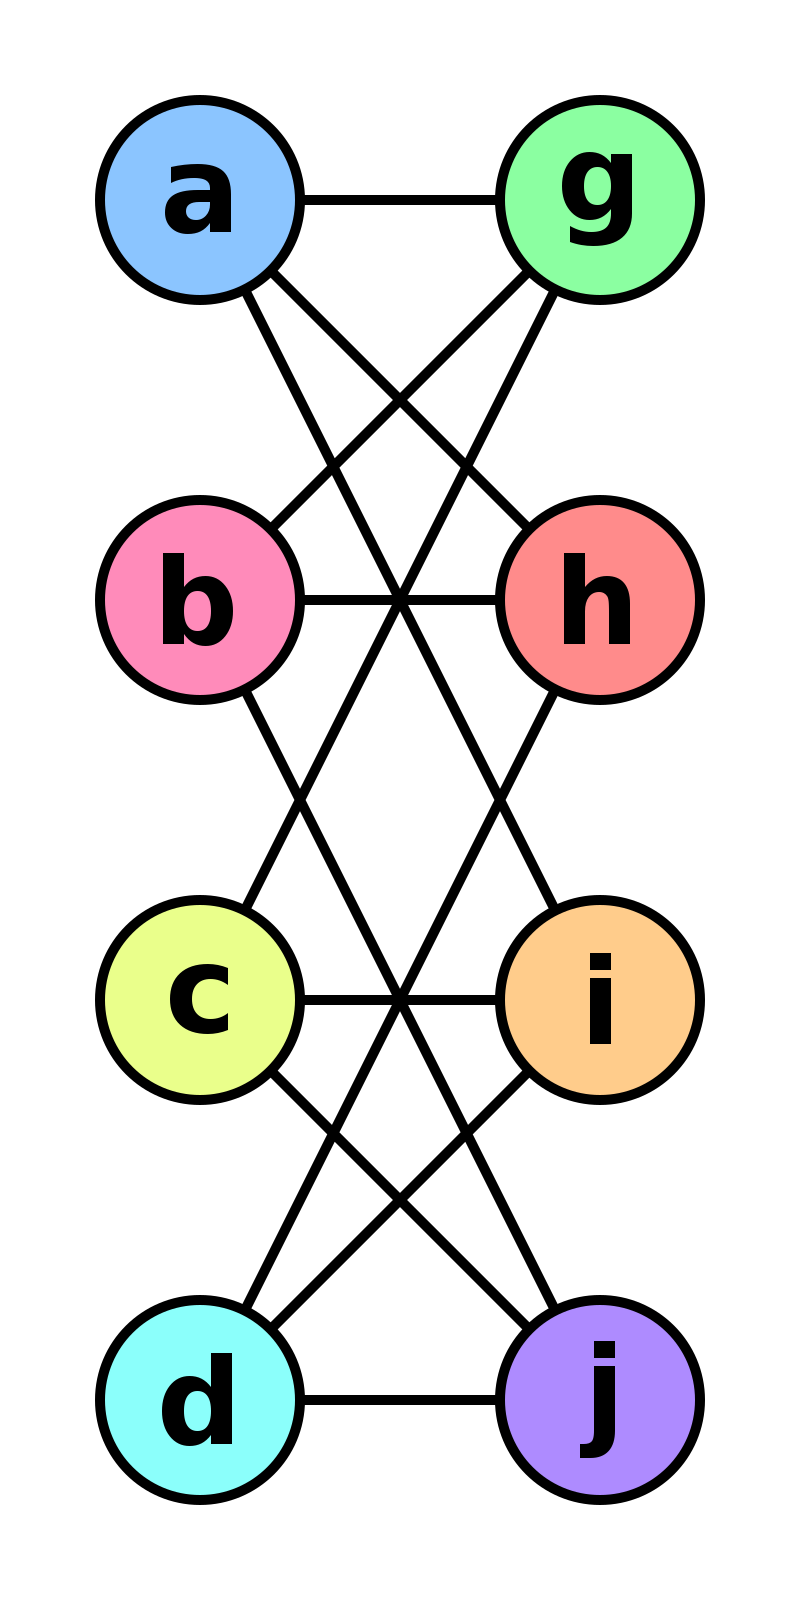
\includegraphics[scale=0.1]{figs/Graph_isomorphism_a.png}
  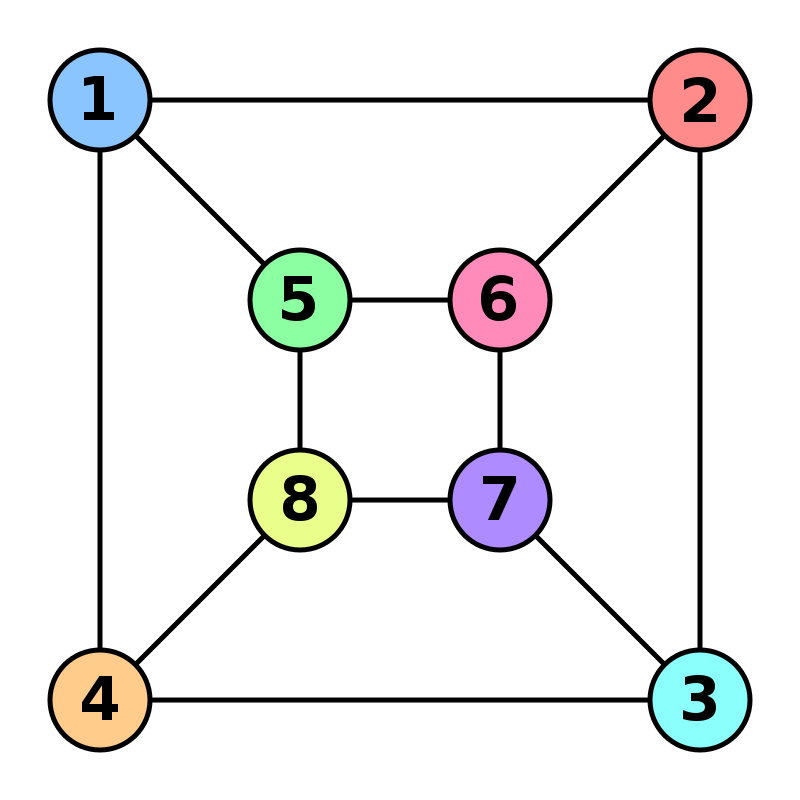
\includegraphics[scale=0.2]{figs/Graph_isomorphism_b.png}

\end{frame}

%---------------------------------------------------------


%---------------------------------------------------------
%Example of the \pause command
\begin{frame}
  \frametitle{图同构的必要不充分条件}
  \begin{center}
    \scalebox{0.8}{
      \begin{minipage}{1\linewidth}
        \begin{algorithm}[H]
        \begin{algorithmic}[1]
        \IF{$V(G) \ne V(H)$}
          \RETURN \FALSE
        \ENDIF
        \FOR{$v$ in $V(G)$ and $V(H)$}
          \STATE $L_v^0 =$ random value
        \ENDFOR
        \FOR{$i=1$ to $|V(G)|$}
          \FOR{$v$ in $V(G)$ and $V(H)$}
            \STATE $L_v^i = hash (\{ L_u^{i-1} : u \in \mathcal{N}(v) \})$
          \ENDFOR
          \IF{the partition of $L_{V(G)}^{i}$ $\ne$ the partition of $L_{V(H)}^{i}$}
            \RETURN \FALSE
          \ENDIF
          \IF{no change in the partition between $L^i$ and $L^{i-1}$ of two grap}
            \STATE \textbf{break}
          \ENDIF
        \ENDFOR
        \RETURN \TRUE
        \end{algorithmic}
        \caption{Weisfeiler-Lehman Test}
        \label{alg:seq}
        \end{algorithm}
      \end{minipage}
      }
  \end{center}
\end{frame}
%---------------------------------------------------------

%---------------------------------------------------------
\begin{frame}

  \frametitle{Weisfeiler-Lehman Test 示例}
  \ctikzfig{figs/WL-1}

\end{frame}
%---------------------------------------------------------

%---------------------------------------------------------
\begin{frame}

  \frametitle{Weisfeiler-Lehman Test 示例}
  \ctikzfig{figs/WL-2}

\end{frame}
%---------------------------------------------------------

%---------------------------------------------------------
\begin{frame}

  \frametitle{Weisfeiler-Lehman Test 示例}
  \ctikzfig{figs/WL-3}

\end{frame}
%---------------------------------------------------------

%---------------------------------------------------------
\begin{frame}

  \frametitle{Weisfeiler-Lehman Test 示例}
  \ctikzfig{figs/WL-4}

\end{frame}
%---------------------------------------------------------

%---------------------------------------------------------
\begin{frame}

  \frametitle{Weisfeiler-Lehman Test 示例}
  \ctikzfig{figs/WL-5}

\end{frame}
%---------------------------------------------------------

%---------------------------------------------------------
\begin{frame}

  \frametitle{Weisfeiler-Lehman Test 示例}
  \ctikzfig{figs/WL-6}

\end{frame}
%---------------------------------------------------------

%---------------------------------------------------------
\begin{frame}

  \frametitle{Weisfeiler-Lehman Test 示例}
  \ctikzfig{figs/WL-7}

\end{frame}
%---------------------------------------------------------

%---------------------------------------------------------
\begin{frame}

  \frametitle{Weisfeiler-Lehman Test 示例}
  \ctikzfig{figs/WL-8}

\end{frame}
%---------------------------------------------------------

%---------------------------------------------------------
\begin{frame}

  \frametitle{Weisfeiler-Lehman Test}
  \begin{block}{WL-Test 解释}
    达到稳定时,图的标签分布是聚合运算的不动点,说明有相同标签的结点
    与其他结点有相似的邻接关系。但标签分布无法决定唯一的邻接关系。
  \end{block}
  \begin{alertblock}{WL-Test 是图同构的必要不充分条件}
    两个同构图经过上述变换后得到的标签分布一定相同,但得到相同的标签分布只能说明两个图\textbf{可能}同构。
  \end{alertblock}
  \ctikzfig{figs/WL-ce}

\end{frame}
%---------------------------------------------------------

\section{图神经网络结构}

%---------------------------------------------------------
\begin{frame}

  \frametitle{基于图数据的任务举例}
  图数据任务隐含了如下假设:结点或图的标签除了与收集的特征有关,还与图的邻接关系有关,故可以通过
  扩展 WL-Test 来设计神经网络。
  \begin{block}{结点分类}
    每个结点 $v \in V$ 都有特征向量 $x_v$ 及对应的标签 $y_v$,
    要求学习每个结点的嵌入向量 $h_v$ 和一种映射 $f$,使得结点的标签可以通过 $\hat{y}_v = f(h_v)$ 预测。
  \end{block}
  \begin{block}{图分类}
    有一系列图 $\{G_1, ..., G_N\}$ 及其标签 $\{y_1, ..., y_N\}$。
    要求学习每个图的嵌入向量 $h_G$ 和一种映射 $g$,使得图的标签可以通过 $\hat{y}_G = g(h_G)$ 预测。
  \end{block}

\end{frame}
%---------------------------------------------------------

%---------------------------------------------------------
\begin{frame}

  \frametitle{图神经网络的计算过程}
    \begin{algorithm}[H]
    \begin{algorithmic}[1]
      \FOR{$v$ in $V(G)$}
        \STATE $h_v^0 = x_v$
      \ENDFOR
      \FOR{$k=1$ to $K$}
        \STATE $a_v^k = AGGREGATE^k(\{h_u^{k-1} : u \in \mathcal{N}(v)\})$
        \STATE $h_v^k = COMBINE^k(h_v^{k-1}, a_v^k)$
      \ENDFOR
      \STATE $h_G = READOUT({h_v^K : v \in G})$
    \end{algorithmic}
    \caption{GNN}
    \label{alg:gnn}
    \end{algorithm}
      
\end{frame}
%---------------------------------------------------------

%---------------------------------------------------------
\begin{frame}

  \frametitle{图神经网络的计算过程}
      
  $AGGREGATE$:聚集邻居结点的信息,如 
  $$a_v^k = MAX(\{RELU(W_a \cdot h_u^{k-1}) : u \in \mathcal{N}(v)\}).$$
  $COMBINE$:引入中心结点的信息,如
  $$h_v^k = W_c \cdot CONCAT(h_v^{k-1}, a_v^k).$$
  在卷积图神经网络中,上述两个过程合为一个:
  $$h_v^k = RELU(W \cdot MEAN \{h_u^{k-1} : u \in \mathcal{N}(v) \cup \{v\} \}).$$
  $READOUT$:聚集结点的嵌入从而生成图的嵌入,如按位取最大值。
\end{frame}
%---------------------------------------------------------

\section{图神经网络的表达能力}

%---------------------------------------------------------
\begin{frame}

  \frametitle{图神经网络与 WL-Test 的比较}
  \begin{block}{定理:图神经网络的表达能力不强于 WL-Test}
    设 $G_1$ 和 $G_2$ 为两个不同构的图,如果一个图神经网络 $\mathcal{A}: \mathcal{G} \rightarrow \mathbb{R}^d$
    将 $G_1$ 和 $G_2$ 映射到不同的嵌入,则 WL-Test 会认为 $G_1$ 和 $G_2$ 不同构。
  \end{block}
  \begin{alertblock}{反例:部分图神经网络的表达能力弱于 WL-Test}
    根源在于 WL-Test 中的哈希函数是单射,而求平均值/最大值/矩阵乘法等操作都不是单射。
  \end{alertblock}
  \ctikzfig{figs/mean-max}

\end{frame}
%---------------------------------------------------------


%---------------------------------------------------------
%Highlighting text
\begin{frame}
\frametitle{Sample frame title}

In this slide, some important text will be
\alert{highlighted} because it's important.
Please, don't abuse it.

\begin{block}{Remark}
Sample text
\end{block}

\begin{alertblock}{Important theorem}
Sample text in red box
\end{alertblock}

\begin{examples}
Sample text in green box. The title of the block is ``Examples".
\end{examples}
\end{frame}
%---------------------------------------------------------


%---------------------------------------------------------
%Two columns
\begin{frame}
\frametitle{Two-column slide}

\begin{columns}

\column{0.5\textwidth}
This is a text in first column.
$$E=mc^2$$
\begin{itemize}
\item First item
\item Second item
\end{itemize}

\column{0.5\textwidth}
This text will be in the second column
and on a second tought this is a nice looking
layout in some cases.
\end{columns}
\end{frame}
%---------------------------------------------------------


\end{document}